\section{Лекция от 24.01.2017}

\epigraph{<<На прошлой лекции Дмитрий Александрович запнулся, на этой посмотрел записи. Ну всё, действительно сложный ТеорВер начался.>>}
{Один из слушателей}

\subsection{Случайные процессы}

\begin{definition}
  Пусть есть множество $T$ (неформально оно обозначает время). Набор случайных
  величин $(x_t, t \in T)$ будем называть \emph{случайным процессом.}
\end{definition}

\begin{remark}
  То, что написано в определении, на самом деле, называется \emph{случайной функцией},
  но для определенности оставим определение в таком же виде, потому что в основном
  будем использовать $T \subseteq \R$, что уже действительно является случайным
  процессом по определению во многих учебниках.
\end{remark}

\begin{definition}
  Классифицируем случайные процессы:
  \begin{itemize}
    \item если $T = \N, \Z, \Z_{+}$ --- случайный процесс с дискретным временем.
    \item если $T = [a, b], \R, \R_{+}$ --- случайный процесс с непрерывным
    временем.
    \item если $T \subseteq \R^d, d > 1$, тогда случайный процесс будет случайным
    полем.
  \end{itemize}
\end{definition}

Сейчас уделим больше внимания дискретным процессам. Будем считать, что у нас
задана тройка Колмогорова $(\Omega, \F, \Pr)$ и все $x_t: \Omega \to \R$.

\begin{definition}
  Для фиксированного $\omega_0 \in \Omega$ функция $\tilde{x}_t(t) = x_t(\omega_0), t \in T$
  является \emph{траекторией} (или \emph{реализацией}) случайного процесса.
\end{definition}

\begin{example}
  $x_t = f(t) \xi$, где $f(t)$ --- какая-то функция, $\xi$ --- случайная величина.
  Приведем пример траекторий для некоторых $\omega_0$.
  \begin{center}
    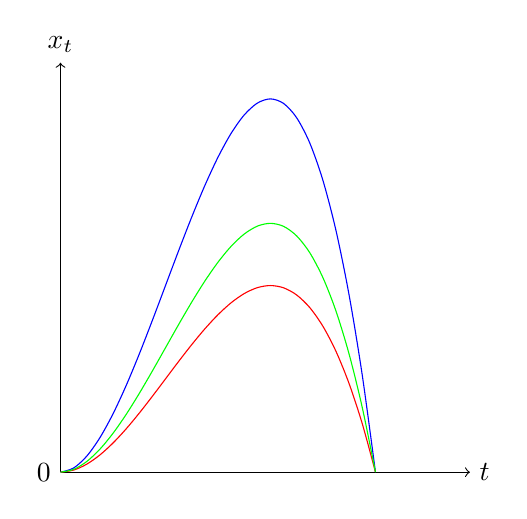
\begin{tikzpicture}
        \draw[->] (0,0) -- (5.2,0) node[right] {$t$};
        \draw[->] (0,0) -- (0,5.2) node[above] {$x_t$};
        \draw (0,0) node[left] {$0$};
        \draw[scale=1,domain=0:4,smooth,variable=\t,blue] plot ({\t},{2*\t*\t - \t*\t*\t/2)});
        \draw[scale=1,domain=0:4,smooth,variable=\x,red] plot ({\x},{\x*\x - \x*\x*\x/4)});
        \draw[scale=1,domain=0:4,smooth,variable=\x,green] plot ({\x},{4*\x*\x/3 - \x*\x*\x/3)});
    \end{tikzpicture}
  \end{center}
\end{example}

\subsection{Случайные блуждания}

\begin{definition}
  Пусть $\{\xi_n, \in \N\}$ --- независимые случайные величины. Определим
  $S_0 = 0$, а $S_n = \xi_1 + \ldots \xi_n, n \in \N$. Тогда $\{S_n, n \in \Z_{+}\}$
  называют \emph{случайным блужданием}.   
\end{definition}

\begin{center}
  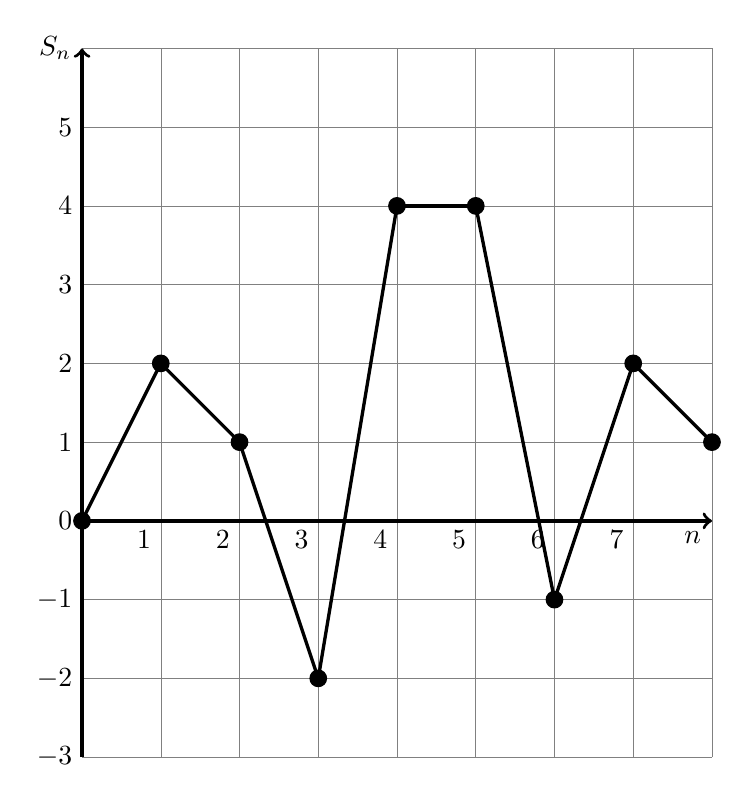
\begin{tikzpicture}
  
  \draw[step=1cm,gray,very thin] (2,-5) grid (10,4);
  \draw[very thick,->] (2,-2) -- (10,-2) node[anchor=north, below left] {$n$};
  \draw[very thick,->] (2,-5) -- (2, 4) node[anchor=east] {$S_n$};

  \node [left] at (2, -5) {$-3$};
  \node [left] at (2, -4) {$-2$};
  \node [left] at (2, -3) {$-1$};
  \node [left] at (2, -1) {$1$};
  \node [left] at (2, 0) {$2$};
  \node [left] at (2, 1) {$3$};
  \node [left] at (2, 2) {$4$};
  \node [left] at (2, 3) {$5$};

  \node [below left] at (3, -2) {$1$};
  \node [below left] at (4, -2) {$2$};
  \node [below left] at (5, -2) {$3$};
  \node [below left] at (6, -2) {$4$};
  \node [below left] at (7, -2) {$5$};
  \node [below left] at (8, -2) {$6$};
  \node [below left] at (9, -2) {$7$};

  
  \node [left] at (2, -2) {$0$};
  
  \draw (2, -2) node[draw,circle,fill=black,minimum size=6pt,inner sep=2pt] (C) {};
  \draw (3, 0) node[draw,circle,fill=black,minimum size=6pt,inner sep=2pt] (C) {};
  \draw (4, -1) node[draw,circle,fill=black,minimum size=6pt,inner sep=2pt] (C) {};
  \draw (5, -4) node[draw,circle,fill=black,minimum size=6pt,inner sep=2pt] (C) {};
  \draw (6, 2) node[draw,circle,fill=black,minimum size=6pt,inner sep=2pt] (C) {};
  \draw (7, 2) node[draw,circle,fill=black,minimum size=6pt,inner sep=2pt] (C) {};
  \draw (8, -3) node[draw,circle,fill=black,minimum size=6pt,inner sep=2pt] (C) {};
  \draw (9, 0) node[draw,circle,fill=black,minimum size=6pt,inner sep=2pt] (C) {};
  \draw (10, -1) node[draw,circle,fill=black,minimum size=6pt,inner sep=2pt] (C) {};

  \draw[very thick, -] (2, -2) -- (3, 0);
  \draw[very thick, -] (3, 0) -- (4, -1);
  \draw[very thick, -] (4, -1) -- (5, -4);
  \draw[very thick, -] (5, -4) -- (6, 2);
  \draw[very thick, -] (6, 2) -- (7, 2);
  \draw[very thick, -] (8, -3) -- (7, 2);
  \draw[very thick, -] (8, -3) -- (9, 0);
  \draw[very thick, -] (10, -1) -- (9, 0);
  \end{tikzpicture}
\end{center}


\begin{example}
  Физической моделью, соответствующую случайному блужданию, могут являться прыжки
  кузнечика.
\end{example}

\subsection{Процесс восстановления}

\begin{definition}

  Пусть $\{\xi_n, n \in \N\}$ --- одинаково распределенные
  неотрицательные случайные величины. Положим $S_0 = 0, S_n = \xi_1 + \ldots \xi_n,
  n \in \N$, а также для каждого $t \geq 0$ рассмотрим такие случайные величины:
  $x_t = \max\{n : S_n \leq t\}$ (если максимума не существует, положим $x_t = +\infty$).

  Процесс $(x_t, t \geq 0)$ называется \emph{процессом восстановления} для
  случайных величин $\{\xi_n, n \in \N\}$.
\end{definition}

График можно описать как-то так для какого-то $\omega_0$:


\begin{center}
  \begin{tikzpicture}
  
  \draw[line width=0.01mm,->] (0, 0) -- (12, 0) node[anchor=north, below left] {$t$};
  \draw[line width=0.01mm,->] (0, 0) -- (0, 7) node[anchor=east] {$x_t$};

  \draw (2.25, 0) node[draw,circle,fill=none,minimum size=4pt,inner sep=2pt] (C) {};
  \draw (5.46, 1) node[draw,circle,fill=none,minimum size=4pt,inner sep=2pt] (C) {};
  \draw (9.8, 2) node[draw,circle,fill=none,minimum size=4pt,inner sep=2pt] (C) {};
  \draw (11.7, 4) node[draw,circle,fill=none,minimum size=4pt,inner sep=2pt] (C) {};

  \draw[very thick, -] (0, 0) -- (2.25, 0);
  \draw[very thick, -] (2.25, 1) -- (5.46, 1);
  \draw[very thick, -] (5.46, 2) -- (9.8, 2);
  \draw[very thick, -] (11.7, 4) -- (9.8, 4);

  \draw[very thick, dashed, -] (0, 1) -- (2.25, 1);
  \draw[very thick, dashed, -] (0, 2) -- (5.46, 2);
  \draw[very thick, dashed, -] (0, 4) -- (9.8, 4);

  \node [left] at (0, 0) {$0$};
  \node [left] at (0, 1) {$1$};
  \node [left] at (0, 2) {$2$};
  \node [left] at (0, 3) {$3$};
  \node [left] at (0, 4) {$4$};

  \node [below] at (2.25, 0) {$S_1$};
  \node [below] at (5.46, 0) {$S_2$};
  \node [below] at (9.8, 0) {$S_3, S_4$};


  \end{tikzpicture}
\end{center}

Где возможны склеивания, как в $S_3, S_4$ --- это лишь означает, что $\xi_4 = 0$.

\begin{example}
  Физической моделью, соответствующую процессу восстановления, может служить
  процесс горения лампочки,
  где $\xi_n$ --- общее время горения $n$-ой лампочки, а $x_t$ тогда будет количеством
  поменянных лампочек до времени $t$.
\end{example}

Пара бы уже что-то доказать. Действительно, покажем, что мы не можем
часто убегать в бесконечность. На самом деле такие ситуации очень плохи в реальной
жизни. Происходит <<перенасыщение>> чего-то. В примере с лампочкой, мы можем менять
бесконечное число лампочек за время ноль. Такая ситуация очень плоха, поэтому,
чтобы успокоиться, докажем следующее утверждение:

\begin{theorem}
  Процесс восстановления конечен с вероятностью один, если $\Pr{\xi = 0} < 1$.
\end{theorem}

\begin{proof}
  Пусть $t > 0$ фиксировано. $\Pr{x_t = +\infty} = \Pr{\forall n : S_n \leq t}$.

  Заметим, что $S_n \leq S_{n + 1}$ из-за неотрицательности $\xi_{n + 1}$.

  Выпишем тривиальное равенство пределов:
  \[
    \lim\limits_{n \to +\infty} \Pr{S_n \leq t} = \lim\limits_{n \to +\infty} \Pr{\frac{S_n}{n} \leq \frac{t}{n}}
  \]

  Есть 2 случая:

  \begin{itemize}
    \item $\E{\xi_i}$ конечно и равно $A > 0$ (больше нуля, так как $\Pr{\xi_i = 0} < 1$).
    Тогда по закону больших чисел имеем,
    что $\frac{S_n}{n} \prto A$ (на самом деле мы немного лукавим, потому что
    в основном курсе эта теорема была доказана с использованием, что все моменты до четвёртого конечны,
    но ЗБЧ работает и при конечности средней величины).

    Тогда продолжим равенство пределов:

    \[
      = \lim\limits_{n \to +\infty} \Pr{\frac{S_n}{n} \leq \frac{t}{n}} \leq
      \lim\limits_{n \to +\infty} \Pr{\frac{S_n}{n} \leq \frac{A}{2}}
    \]

    Действительно, с какого-то момента $\frac{t}{n} < \frac{A}{2}$, так как
    $A > 0$. Далее, из закона больших чисел получаем:

    \[
      = \lim\limits_{n \to +\infty} \Pr{A \leq \frac{A}{2}} = 0.
    \]

    Последнее равенство идёт из-за неотрицательности $A$.

    Поэтому $\Pr{x_t = +\infty} = 0$ в этом случае.

    \item $\E{\xi_i} = +\infty$.

    Рассмотрим $\hat{\xi}_i = \min(\xi_i, 1) \leq \xi_i$. Откуда сразу получаем,
    что $\hat{S}_n = \hat{\xi}_1 + \ldots + \hat{\xi}_n \leq S_n$.

    Заметим, что $\E{\hat{S}_n}$ конечно, так как матожидание каждого из
    $\hat{\xi}_i$ конечно (так как $\hat{\xi}_i \leq 1$).

    А значит, что $\Pr{S_n \leq t} \leq \Pr{\hat{S}_n \leq t}$ (так как
    $S_n \geq \hat{S}_n$, а значит, что $\hat{S}_n$ принимает меньшие значения).

    Но мы уже всё доказали для конечного матожидания $\hat{\xi}_i$, поэтому получаем,
    что $\Pr{\hat{S}_n \leq t} \to 0$, откуда и $\Pr{S_n \leq t} \to 0$, что нам и требуется.
  \end{itemize}

\end{proof}

Приведём более мощный пример, обобщим эту модель.

\begin{example}
  Пусть $\{\xi_n, n \in \N\}$ --- независимые и одинаково распределенные
  случайные величины, $\{\eta_n, n \in \N\}$ --- независимые и одинаково
  распределенные случайные величины, притом независимы с $\{\xi_n, n \in \N\}$.

  Пусть $(x_t, t > 0)$ --- процесс восстановления, то есть
  $x_t = \max\{n : \xi_1 + \ldots + \xi_n \leq t\}$.

  Для $y_0, c > 0 \in \R$ введём

  \[
    Y_t = y_0 + ct - \sum\limits_{k = 1}^{x_t} \eta_k
  \]

  Эту модель называют моделью страхования Спарре-Андресена. Поясним, что значит
  каждая введенная переменная/величина.

  \begin{itemize}
    \item $y_0$ --- начальный капитал.
    \item $c$ --- скорость поступления страховых взносов. Для простоты считают,
    поступление линейно, что примерно одинаково <<бьются>> машины в любое время
    года.
    \item $\eta_k$ --- размер выплаты с номером $k$.
    \item $\xi_k$ --- время между $k - 1$-й и $k$-й выплатой.
    \item $x_t$ --- количество выплат к моменту времени $t$.
    \item $\sum\limits_{k = 1}^{x_t} \eta_k$ --- общий объём выплат по времени.
    \item И понятно, что тогда $Y_t$ --- текущий капитал.
  \end{itemize}

  В будущем, когда в нашем курсе мы затронем мартингалы, мы сможем понять и
  оценить, какова вероятность, что компания разорится.

  Ясно, что тогда график капитала от времени будет выглядеть примерно 
  таким образом:


\begin{center}
  \begin{tikzpicture}

  \draw[line width=0.01mm,->] (0, 0) -- (13, 0) node[anchor=north, below left] {$t$};
  \draw[line width=0.01mm,->] (0, 0) -- (0, 7) node[anchor=east] {$Y_t$};

  \draw[very thick, ->] (0, 2) -- (2, 5);
  \draw[very thick, dashed, -] (2, 5) -- (2, 2);
  \draw[very thick, ->] (2, 2) -- (3, 3.5);
  \draw[very thick, dashed, -] (3, 3.5) -- (3, 1);
  \draw[very thick, ->] (3, 1) -- (7, 7);
  \draw[very thick, dashed, -] (7, 7) -- (7, 5);
  \draw[very thick, ->] (7, 5) -- (7.8, 6.2);
  \draw[very thick, dashed, -] (7.8, 6.2) -- (7.8, 4.5);
  \draw[very thick, ->] (7.8, 4.5) -- (8.8, 6);

  \node [left] at (0, 2) {$y_0$};
  
  \node [below] at (2, 0) {$S_1$};
  \node [below] at (3, 0) {$S_2$};
  \node [below] at (7, 0) {$S_3$};
  \node [below] at (7.8, 0) {$S_4$};


  \end{tikzpicture}
\end{center}
\end{example}

\subsection{Простые случайные блуждания}

\begin{definition}
  Пусть $\{\xi_n, n \in \N\}$ независимые одинаково распределенные случайные
  величины такие, что для какого-то $p \in [0, 1]$
  \[
    \Pr{\xi_n = 1} = p, \Pr{\xi_n = -1} = 1 - p = q
  \]
  Положим $S_0 = 0, S_n = \xi_1 + \ldots \xi_n,
  n \in \N$. Тогда $\{S_n, n \in \Z_{+}\}$ называют \emph{простым случайным
  блужданием на прямой}.
\end{definition}

Смысл этого определения в том, что на каждом шаге мы выбираем с какими-то вероятностями, в какую сторону пойти.

Понятное дело, что этим можно не ограничиваться и, например, ходить в 4 разные
стороны на плоскости. Но давайте пока разберёмся с одномерным случаем.

\begin{definition}
  Если $p = q = \frac{1}{2}$, то говорят, что случайное блуждание симметрично.
\end{definition}

\begin{remark}
  Не лишним будет упомянуть, что в данном случае $\E{S_n} = (p - q)n$. 
  Действительно, если раскрыть по линейности, то совершенно ясно по 
  определению, что $\E{\xi_i} = p - q$.
\end{remark}

Перед нами возникают достаточно интересные вопросы:

\begin{itemize}
  \item[1.] Какова вероятность вернуться в ноль после ненулевого количества шагов?
  \item[2.] Какое среднее время мы проведем в нуле? 
  То есть сколько в среднем раз мы окажемся в нуле при достаточно больших $n$.
  \item[3.] Геометрия траекторий. То есть то, как выглядит график, какие существуют зависимости.
  Нашей кульминацией на этот вопрос будет закон повторного логарифма, который показывает,
  насколько далеко в среднем мы можем отходить от нуля.
\end{itemize}

Будем постепенно на все эти вопросы отвечать. Каждый из них --- отдельная
история, поэтому будем отвечать постепенно.

\subsection{Возвращение в ноль в простом случайном блуждании}

Легко понять, что нас интересует $\Pr{\exists \ n > 0 : S_n = 0}$.

Попробуем найти $\Pr{S_n = x}$. Во-первых, ясно, что $n$ и $x$ должны
быть одной четности, так как иначе мы не сможем из нуля прийти в $x$.
Также, нужно, чтобы $n \geq |x|$, иначе мы просто не дойдём до 
$x$, но скомпенсируем в будущем это тем, что $\binom{n}{k} = 0$ при $k > n$.

Пусть мы сделали $k$ шагов вправо и $n - k$ шагов влево. Под шагами 
подразумевается $+1$ и $-1$ соответственно. Тогда ясно, что
$k = \frac{n + x}{2}$, так как должно выполняться равенство $k - n + k = x$.

Поэтому получаем из-за того, что нам надо выбрать $k$ ходов, ответ для данной вероятности:

\[
  \Pr{S_n = x} = \binom{n}{k}p^kq^{n - k}I\{n + x \text{ чётно}\}
\]

Но этого мало. Мы не сможем как-то легко посчитать вероятность существования $n$, что $S_n = 0$.

Поэтому мы хотим понять, когда впервые достигнем нуля. Ясное дело, что нуля 
можно достигнуть только на четных ходах. Поэтому давайте посчитаем такую
вероятность:

\[
  \Pr{S_1 \neq 0, \ldots, S_{2n - 1} \neq 0, S_{2n} = 0}
\]

Заметим, что все $S_1, \ldots, S_{2n - 1}$ либо одновременно больше нуля,
либо все одновременно меньше нуля, так как из-за дискретной непрерывности,
если есть $S_i, S_j$ разных знаков, то найдётся между ними ноль, что 
противоречит тому, что мы ищем. 
Так как нам надо сделать $n$ ходов вправо и влево, эти случаи ничем не отличаются. Посчитаем вероятность, когда все $S_i > 0, i \in [2n - 1]$.

Посмотрим на траектории, которые у нас могут получиться:

\begin{center}
  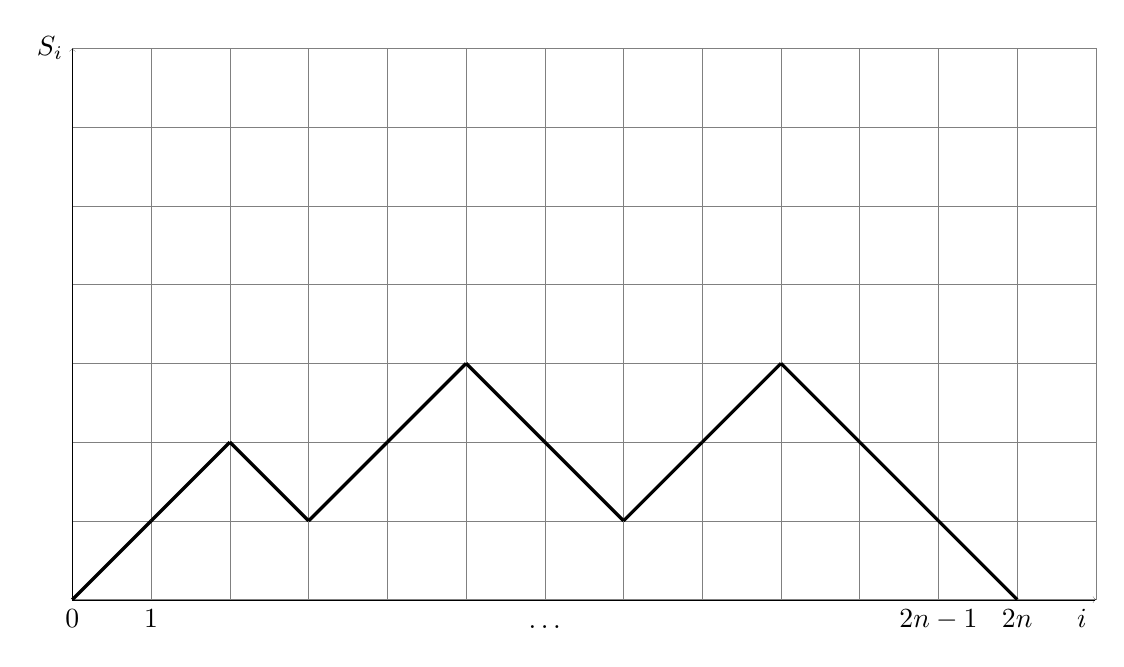
\begin{tikzpicture}

  \draw[step=1cm,gray,very thin] (0,0) grid (13,7);
  \draw[line width=0.01mm,->] (0, 0) -- (13, 0) node[anchor=north, below left] {$i$};
  \draw[line width=0.01mm,->] (0, 0) -- (0, 7) node[anchor=east] {$S_i$};


  \draw[very thick, -] (0, 0) -- (1, 1);
  \draw[very thick, -] (1, 1) -- (2, 2);
  \draw[very thick, -] (2, 2) -- (3, 1);
  \draw[very thick, -] (3, 1) -- (4, 2);
  \draw[very thick, -] (4, 2) -- (5, 3);
  \draw[very thick, -] (5, 3) -- (6, 2);
  \draw[very thick, -] (6, 2) -- (7, 1);
  \draw[very thick, -] (7, 1) -- (8, 2);
  \draw[very thick, -] (8, 2) -- (9, 3);
  \draw[very thick, -] (9, 3) -- (10, 2);
  \draw[very thick, -] (10, 2) -- (11, 1);
  \draw[very thick, -] (11, 1) -- (12, 0);

  \node [below] at (0, 0) {$0$};
  \node [below] at (1, 0) {$1$};
  \node [below] at (6, -0.2) {$\dots$};
  \node [below] at (11, 0) {${2n - 1}$};
  \node [below] at (12, 0) {${2n}$};
  \end{tikzpicture}
\end{center}

Теперь мы хотим посчитать все такие пути.

Обозначим через $\epsilon_i$ --- выбор $\pm1$ на $i$-ом шаге. Тогда путь подходит 
тогда и только тогда, когда $\sum\limits_{i = 1}^{2n} \epsilon_i = 0$ и
$\sum\limits_{i = 1}^{k} \epsilon_i > 0, k \in [2n - 1]$.

Обозначим количество таких путей через $\tilde{C}_n$.

А теперь вспомним, что числа Каталана задаются практически так же. Те, кто 
ходил на курс дискретной математики, помнят, что есть соответствие между 
числами Каталана и количеством путей, отвечающим свойствам: $\sum\limits_{i = 1}^{
2n} \epsilon_i = 0$ и
$\sum\limits_{i = 1}^{k} \epsilon_i \geq 0, k \in [2n - 1]$.

Обозначим количество таких путей через $C_n$.

\begin{lemma}
  $\tilde{C}_{n + 1} = C_{n}.$
\end{lemma}

\begin{proof}
  Рассмотрим любой путь, соответствующий $\tilde{C}_{n + 1}$. Заметим, что
  первые и последние шаги обязательно $+1$ и $-1$ соответственно. Поэтому, 
  при <<поднятии>> оси $Oi$ мы получим, что перед нами путь из $C_n$, 
  действительно, это так, так как префиксные суммы уменьшились на 1 и не стали 
  отрицательными, а сумма по-прежнему сохранилась нулевая.

  В другую сторону доказывается аналогично. См. иллюстрацию.

  \begin{center}
  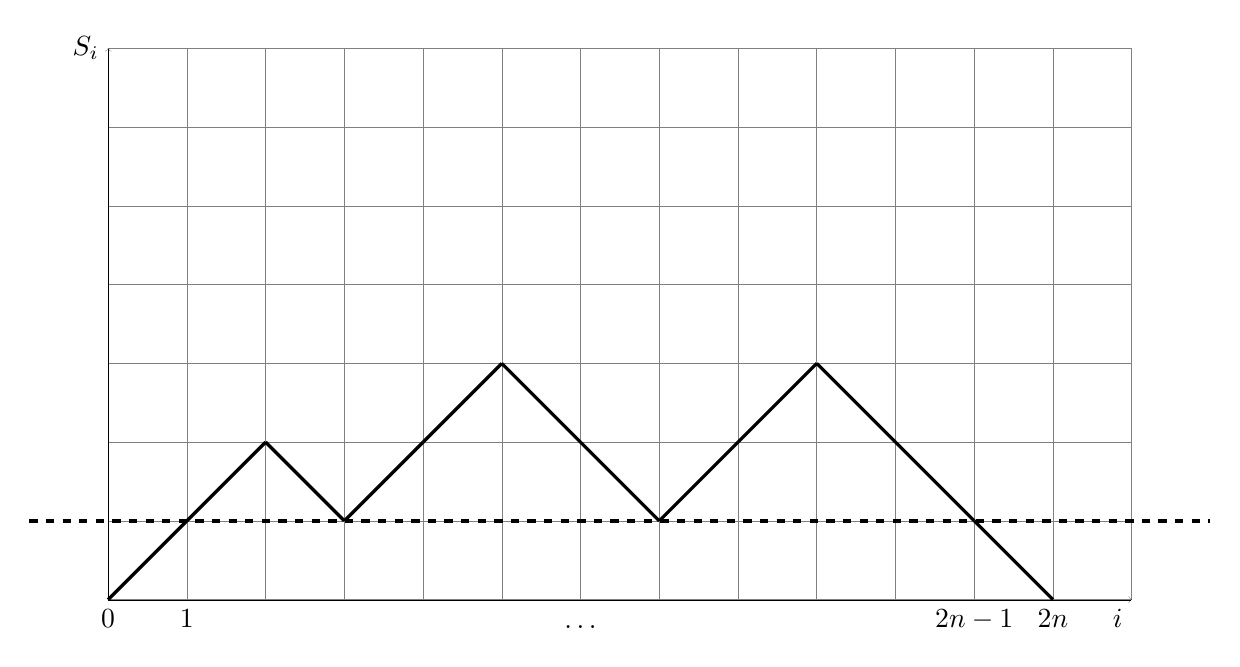
\begin{tikzpicture}

  \draw[step=1cm,gray,very thin] (0,0) grid (13,7);
  \draw[line width=0.01mm,->] (0, 0) -- (13, 0) node[anchor=north, below left] {$i$};
  \draw[line width=0.01mm,->] (0, 0) -- (0, 7) node[anchor=east] {$S_i$};


  \draw[very thick, -] (0, 0) -- (1, 1);
  \draw[very thick, -] (1, 1) -- (2, 2);
  \draw[very thick, -] (2, 2) -- (3, 1);
  \draw[very thick, -] (3, 1) -- (4, 2);
  \draw[very thick, -] (4, 2) -- (5, 3);
  \draw[very thick, -] (5, 3) -- (6, 2);
  \draw[very thick, -] (6, 2) -- (7, 1);
  \draw[very thick, -] (7, 1) -- (8, 2);
  \draw[very thick, -] (8, 2) -- (9, 3);
  \draw[very thick, -] (9, 3) -- (10, 2);
  \draw[very thick, -] (10, 2) -- (11, 1);
  \draw[very thick, -] (11, 1) -- (12, 0);
  \draw[very thick, dashed, -] (-1, 1) -- (14, 1);


  \node [below] at (0, 0) {$0$};
  \node [below] at (1, 0) {$1$};
  \node [below] at (6, -0.2) {$\dots$};
  \node [below] at (11, 0) {${2n - 1}$};
  \node [below] at (12, 0) {${2n}$};
  \end{tikzpicture}
\end{center}
\end{proof}

Получается, что

\[
  \Pr{S_1 > 0, \ldots, S_{2n - 1} > 0, S_{2n} = 0} = C_{n - 1}(pq)^n
\]

И соответственно:

\[
  \Pr{S_1 \neq 0, \ldots, S_{2n - 1} \neq 0, S_{2n} = 0} = 2C_{n - 1}(pq)^n
\]

Внимательный читатель заметит, что чтобы посчитать самую исходную 
вероятность, надо просто сложить все такие выше. О том, как такие вещи 
складывать (в частности о характеристических функциях), мы поговорим в
следующей лекции.

